\setstretch{2}
\section{Chapter Summary}
\section{FAD as a marker for metabolic health in the retina}
Mapping the concentration of FAD would enable the diagnosis of retinal disease before physical damage to eyesight develops, at the stage of metabolic dysfunction. FAD is a flavoprotein produced in the body as a by-product of oxygen metabolisation from aerobic respiration (\cref{eq:resp})~\cite{berg2007biochemistry} to create ATP - the bodies source of energy. In the formation of retinal disease, the retina would exhibit abnormal metabolic activity - ATP usage - and would present in the retina as areas with abnormal FAD distribution.
\begin{equation}\label{eq:resp}
    \ce{C6H12O6 + 6O2 -> 6CO2 + 6H2O + ATP}
\end{equation}
While the magnitude of the changes in retinal FAD distribution associated with retinal disease is not know attempts can be made to detect the presence of FAD and assess it feasibility as a diagnostic tool. Changes in FAD concentration can be anaesthetised in animal models by artificially restricting systemic oxygen consumption producing a detectable change in the SFLIM measurements. In normoxic conditions, (\qty{21}{\percent}\ce{FiO2}, oxygen metabolism is typical however in hypoxic conditions (\qty{15}{\percent}\ce{FiO2}) the retina is starved of oxygen thus lowering the detectable concentration of FAD. After death when all metabolic processes have cease the concentration of FAD should tend to zero - in rat cortexes this has been reported as the FAD leaking out of arteries forming `halos'~\cite{martinez2017understanding}.
In this chapter, the SFLIO device (described in~\cref{chap:fliodevice}) was used to record \textit{in-vivo} SFLIM images of the retinas of anaesthetised rats under normoxic, hypoxic, and post-mortem conditions where the concentration of retinal FAD is recovered using the SFLIM unmixing algorithm (described in \cref{chap:tensSFLIM}). Successful detection of FAD is then signified by the changes in the recovered retinal FAD concentration being compatible with what is expected with aerobic respiration. Finally, from this a feasibility of quantifying retinal FAD in human retinas can explored.
\subsection{Estimating The Change in Retinal FAD Concentration at Hypoxia}
The expected variation in FAD concentration as a response to changing oxygenation can be modelled by estimating the rate of FAD production due to oxygen metabolisation in the retina at both normoxia, and hypoxia.
The rate at which oxygen is metabolised $Q_{\ce{O2}}$ is calculated using~\cref{eq:O2rate} from the average rate of blood flow through the ophthalmic artery, $Q_{ret}$, and the relative change in saturation of blood entering, ${S\ce{O2}}_{in}$, and exiting, ${S\ce{O2}}_{out}$, it.
\begin{equation}\label{eq:O2rate}
    Q_{\ce{O2}} = Q_{ret}({S\ce{O2}}_{in}-{S\ce{O2}}_{out})H
\end{equation}
The rate of blood flow through the ophthalmic artery was taken as $Q_{ret} = \qty{41.35}{\micro\litre\per\minute}$ by averaging two reported measurements in literature~\cite{dai2013absolute,riva1985blood}. The oxygen saturation - the ratio of oxygenation to deoxygenated haemoglobin in the blood - has been reported as \qty{92.20}{\percent} and \qty{55.60}{\percent} for blood entering and exiting the ophthalmic artery~\cite{dunn2016physiology}. Using~\cref{eq:O2rate} the rate of oxygen metabolisation was estimated to be $Q_{\ce{O2}}=\SI{3.155}{\micro\litre\per\minute}$ where $H=\num{0.2085}$ is H{\"u}ffners constant which is the volumetric ratio of oxygen to haemoglobin in the blood~\cite{dunn2016physiology}. 
The rate of FAD production, $Q_{FAD}$, can then be determined by considering that for every metabolised \ce{O2} molecule $k_{FAD} = 3$ molecules of FAD are produced with an efficiency of $\eta_{FAD} = \qty{1.3}{\percent}$~\cite{berg2007biochemistry,ames1992energy}.
\begin{equation}
    Q_{FAD} = Q_{\ce{O2}}k_{FAD}\eta_{FAD}
\end{equation}
This yields a production rate of $Q_{FAD} = \qty{0.123}{\micro\litre\per\min}$ which is then be converted to a steady state volume of FAD by assuming that all FAD in the retina is produced in the time taken for blood to flow through the retina and any FAD that is consumed is replaced upon the next circulation period of blood. With a blood flow period of $\delta T = \qty{4.7}{\second}\equiv \qty{0.078}{\minute}$ measured as the time interval between blood entering and exiting the ophthalmic artery~\cite{khoobehi1990measurement}.
\begin{equation}
    V_{FAD} = Q_{FAD}\delta T
\end{equation}
With this calculated volume of retinal FAD,$V_{FAD} = \qty{9.639}{\nano\litre}$, corresponds to $N_{FAD} = \qty{12.27}{\nano\mole}$ using~\cref{eq:nummoles} with a $gfm_{FAD} = \qty{785.56}{\gram\per\mole}$, a density equal to that of water of $\rho_{FAD} = \qty{1}{\gram\per\milli\litre}$, and $N_{A} = \qty{6.022e23}{\per\mole}$.
\begin{equation}\label{eq:nummoles}
    N_{FAD} = V_{FAD}\rho_{FAD}gfm_{FAD}
\end{equation}
Finally, the result of~\cref{eq:nummoles} is expressed as a concentration by approximating the retina as a cuboid with thickness of \qty{344}{\um} and surface area of \qty{1361}{\milli\metre\squared} to estimate its volume~\cite{nagra2017determination,myers2015retinal}.
\begin{equation}\label{eq:FADconc}
    C_{FAD} = \frac{N_{FAD}}{V_{ret}} = \SI{26.9921}{\micro\mole\per\litre}
\end{equation}
While this analysis does represent a simplified interpretation of the biological functions in the retina it is commensurate with reported measurements of flavoproteins in rabbit eye's. In~\citeauthor{batey1991analysis}\cite{batey1991analysis}, the concentration is defined as \qty{39.3}{\pico\mole\per\milli\gram} by weight of the retina which is within \qty{10}{\percent} of the estimation above when converted to equivalent units - $C_{FAD} = \qty{37.64}{\pico\mole\per\milli\gram}$ obtained using the result of \cref{eq:nummoles} and taking the mass of the retina as \qty{326}{\milli\gram}~\cite{batey1991analysis,feke1989blood}.
\\
The volume of FAD in the retina at hypoxia can then be estimated by assuming that the drop in maximal oxygen consumption, ${\dot{V}\ce{O2}}_{max}$, due to hypoxia will induce a decrease in the volume of retinal FAD of an equal order. This rate of maximal oxygen consumption was measured of sedentary and endurance trained subjects as reported in~\citeauthor{ferretti1997decrease}\cite{ferretti1997decrease} and shown in \cref{tab:VO2max}. 

\begin{table}[htb]
    \centering
    \begin{tabular}{|c|c|c|}
    \hline
    \ce{FiO2} & \multicolumn{2}{c|}{${\dot{V}\ce{O2}}_{max}$ (\si{\litre\per\minute})}\\
    \cline{2-3}
    & Sedentary & Athletic\\
    \hline
    \qty{21}{\percent} & \num{3.13} & \num{4.11}\\
    \qty{13}{\percent} & \num{2.27} & \num{2.92}\\
    \hline
    \end{tabular}
    \caption{In \citeauthor{ferretti1997decrease}\cite{ferretti1997decrease}, the maximal rate of oxygen consumption was measured of sedantary subjects and subject with a background in endurance sports for a range of inspired oxygen concentrations (\ce{FiO2}). Reproduced from Table. 1 of \citeauthor{ferretti1997decrease}\cite{ferretti1997decrease}.}
    \label{tab:VO2max}
\end{table}
The ratio between the hypoxic and normoxic measurements of ${\dot{V}\ce{O2}}_{max}$ are then $\Gamma = \num{0.725}$, and $\Gamma = \num{0.710}$ for sedentary and athletic subjects, receptively. Taking the case of a sedentary subject the volume of FAD at hypoxia is $V_{FAD,hypoxia} = \Gamma V_{FAD, normoxia} = \qty{6.839}{\micro\litre}$ and the concentration of FAD at hypoxia is estimated as $C_{FAD,hypoxia} = \Gamma C_{FAD, normoxia} = \qty{19.164}{\micro\mole\per\litre}$. \\
In the SFLIM measurements of anaesthetised, hypoxic, rats, the relative mean concentration of FAD it would be expected to be on-the-order of \qty{30}{\percent} lower than the recorded FAD concentration measured of normoxic rats. Although measurements of the concentration of retinal FAD, nor measurements of oxygen saturation in the for hypoxia and normoxic retinas have not been reported for rats this analysis is still useful for confirming that FAD concentration would be expected to decrease under acute hypoxia (\ce{FiO2}) \qty{15}{\percent}. In humans, the decrease of oxygen saturation in the retina, due to acute hypoxia, was reported by \citeauthor{choudhary2013assessment}\cite{choudhary2013assessment}, as \qty{8.2}{\percent} and \qty{8.3}{\percent} for arterial and venous blood, respectively. From this, it could be concluded that a decrease in retinal FAD of $\approx\qty{8}{\percent}$ would be expected due to acute hypoxia. However, as a result of acute hypoxia in humans, the retinal blood vessels dilate by a factor of between \qtyrange{3.5}{21}{\percent}\cite{choudhary2013assessment,frayser1971response} and according to Poiseuille's Law (\cref{eq:poislaw})~\cite{westerhof2019law}.
\begin{equation}\label{eq:poislaw}
    \Delta P \propto  \frac{Q}{r^{4}}
\end{equation}
This causes a fourth-power increase in the rate of blood flow, $Q$, assuming equal blood pressure, $\Delta P$, for an increasing radius of blood vessel, $r$. For the above dilation factors this would represent an increase in venous blood flow of \qtyrange{16}{114}{\percent}. The affect of increased venous blood flow could imply the concentration of retinal FAD would paradoxically increase as a result of acute hypoxia. This underpins the need for quantitative measurements of retinal fluorophores such as those carried out and presented in this chapter.
\FloatBarrier
\section{\textit{In-Vivo} SFLIM Measurements of Anaesthetised Rats}
\subsection{Experimental Protocol}
The reported imaging experiments were carried out in the labs of Prof. Kenneth J. Smith (Institute of Neuroinflammation, UCL) where Helen Yang (Institute of Neuroinflammation, UCL) prepared the rats for imaging, administered isoflurane to anaesthetise them, and monitored health throughout the imaging session. An external nitrogen supply was mixed with room-air and fed into a fitted nose-cone to control the fraction of inspired oxygen between . Albino rats were chosen for their lack of melanin in the eye which reduces the loss of emitted retinal autofluorescence to absorption and maximising SNR in detected fluorescence. As shown in~\cref{fig:ratsetup}, the rat is secured to the imaging platform and the pupil is dilated using Tropicamide drops to increase pupil diameter (\qtyrange{1.20}{4.35}{\mm}~\cite{himmel2019pupillary}) - maximising the number of detected photons. The eye lids are fixed open with stitches and contact lens is fitted to index-match the rats eye lens. Viscotears gel is applied around the cornea to prevent the eye becoming dry and irritated - inducing additional eye movement and motion requiring correction. To accommodate the rats smaller eyeball diameter, of \SI{6.3}{\mm}~\cite{pazos2015rat}, a field-lens ($\varphi = 2''$, $f = \SI{85}{\mm}$) is fitted to the objective lens of the fundus camera. This additional lens did induce reflections from the illumination source off the front surface of the objective lens and rear surface of the field lens degrading some of the brightfield images with glare (\cref{fig:Ratscmosimages}a) with the penalty of reducing the effectiveness of the motion detection process. This glare was observed to be independent of the motion of the retina which would cause errors in the detected motion in the phase-cross correlation process. By multiplying the images by a mask that is zero in the glare-affected areas and unity elsewhere, the effects of glare was satisfactorily mitigated.  Alternatively, the glare could be removed using an image recorded of a non-reflective scene containing only the glare ($I_{dark}$) and linearly subtracting it from an recorded image ($I_{raw}$) to produce a glare-free image: $I = \alpha I_{raw} - I_{dark}$. 


\begin{figure}
    \centering
    \begin{annotatedFigure}{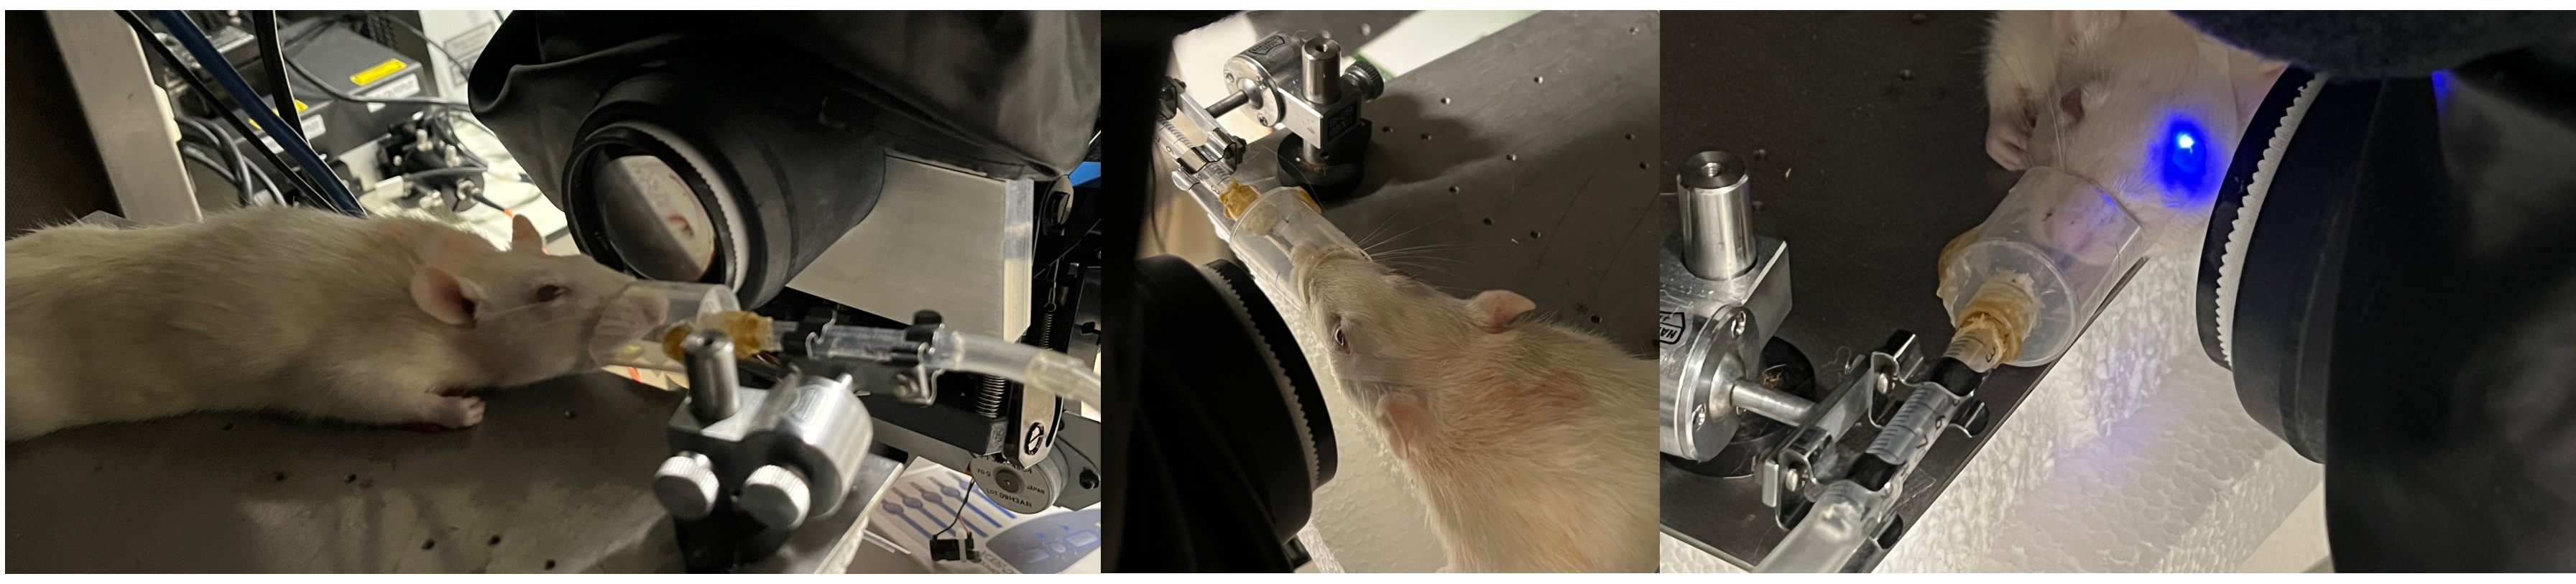
\includegraphics[width = \textwidth]{figures/ratUCL/RatSetupFigure.pdf}}
        \annotatedFigureText{0.015,0.83}{white}{0.3}{a)}
        \annotatedFigureText{0.435,0.83}{white}{0.3}{b)}
        \annotatedFigureText{0.66,0.83}{white}{0.3}{c)}
    \end{annotatedFigure}
    
    \caption{a) and b) The anaesthetised rat is positioned on the imaging platform perpendicular to the SFLIO system to have the rat's retina parallel with the image plane. The fundus camera is moved axially such that the illumination forms a focussed spot on the cornea - evenly illuminating the retina (c).}
    \label{fig:ratsetup}
\end{figure}
Two rats were imaged over three days. For each acquisition brightfield images are recorded continuously (\SI{50}{\ms} exposure at \SI{10}{\Hz}) in tandem with the FLIMera operating in raw mode over a two minute acquisition period for all 5 spectral filters. Due to the large file size generated from the FLIMera RAW acquisition around \SI{10}{\minute} is required the build and save the \SI{50}{\giga\byte} stream of photon counts for each spectral channel. This SFLIM acquisition is carried out while the rats are cycled from normoxia to hypoxia (\SI{15}{\percent}\ce{FiO2}) and then back to normoxia again with an $\approx 5$~minute interval between each acquisition. These intervals between spectral filters and oxygenation states minimises any photobleaching and should ensure that metabolic processes and FAD concentration re-stabilise although long periods of hypoxia can cause the rat to die due to oxidative stress. SFLIM images were recorded for the first rat on the second day. As before (\cref{fig:flimerascmossync}), the two detectors are synchronised in time by initially having the laser shutter closed at the start of the acquisition and then opening it after a short period of time and detecting the Heaviside-like change in photon flux. Due to the anaesthetic the nervous response in the rats is suppressed which eliminates any visible saccades in the image sequence. The motion correction algorithm developed in \cref{chap:motionreg} is still utilised to ensure any small movements of the rat over the hour long imaging sessions does not cause misalignment between spectral filters. However due to the no pixel super-sampling was performed (\cref{fig:FLIMerareg}c).

\begin{figure}
    \centering
    \begin{annotatedFigure}{\includegraphics[width = \textwidth]{figures/ratUCL/RatsCMOSfigure.pdf}}
        \annotatedFigureText{0.025,0.91}{white}{0.3}{a)}
        \annotatedFigureText{0.35,0.91}{white}{0.3}{b)}
        \annotatedFigureText{0.68,0.91}{white}{0.3}{c)}
        \annotatedFigureText{0.19,0.425}{white}{0.3}{d)}
        \annotatedFigureText{0.52,0.425}{white}{0.3}{e)}
    \end{annotatedFigure}
    \caption{a - c) Shows example brightfield images recorded of each of the 3 rats imaged. Each frame is recorded over an integration time of \SI{30}{\ms} at a rate of \SI{10}{\Hz} where a small amount of glare is present in the highlighted region of a). In d) and e) a fluorescence intensity image was recorded using a \SI{500}{\nm} long-pass filter over integration times of \SI{1}{\second} and \SI{5}{\second} respectively.}
    \label{fig:Ratscmosimages}
\end{figure}
\FloatBarrier
\subsection{Detected Translational Motion in Rat Retinas}
As discussed in \cref{chap:motionreg}, compensation of retinal motion is required for producing a high-contrast image where the vasculature is sharply defined. This would enable any variation in the distribution of FAD in the retina to be resolved with high confidence. Retinal motion is detected from image sequences by computing the phase-cross correlation between a reference image and each successive frame in the sequence - where this reference image is the first fully illuminated frame in the sequence after the laser shutter has been opened. This process was carried out for each spectral channel in the SFLIM acquisition and it was found a simple model of translational motion was sufficient for producing a brightfield image free of motion artefacts (see figure). 

However, in one instance the rat exhibited laboured breathing causing motion that cannot simply be described by simple translations in the horizontal and vertical axis. The accuracy of recovered fluorophores would be affected by this but could have been mitigated by using a more flexible motion detection algorithm which could account for non-affine or non-rigid motion.
\begin{figure}
    \centering
    \includegraphics[width = 0.9\linewidth]{figures/ratUCL/RatMotionFigure.pdf}
    \caption{Montage of brightfield image sequence recorded at normoxia after the rat had previously been acutely hypoxia (\SI{12}{\percent}\ce{FiO2}) for a period. Laboured breathing in the rat caused artefacts in the sequence as show above. This is better resolved by viewing the supplementary video ``Rat3BreathingMotion''. This motion is correctable using the existing motion correction algorithm discussed elsewhere \cref{fig:ratbreathcorrection}}
    \label{fig:ratbreathmotion}
\end{figure}
\begin{figure}
    \centering
    \includegraphics[width=0.9\linewidth]{figures/ratUCL/RatBreathCorrection.pdf}
    \caption{Caption}
    \label{fig:ratbreathcorrection}
\end{figure}

\textcolor{red}{TO DO: Write caption for other figure and create video file of the breathing motion}
\FloatBarrier
\subsection{Addressing Lack of Spatial Variaton in SPAD Images}

\FloatBarrier
\section{Recovering FAD Concentration Using SFLIM Unmixing}

\FloatBarrier
\subsection{Darkfield Correction}
\FloatBarrier
\subsection{Recovered Distribution of Retinal Fluorophores}
\FloatBarrier
\section{Correlating Variations in FAD to Changes in Oxygenation}
\FloatBarrier
\subsection{Assessing Statistical Significance of FAD Response}
\FloatBarrier
\subsection{Comparing Detected Changes with PCA and Spectral Angle Maps}
\FloatBarrier
\section{Conclusions}
\section{Future Work and Experimental Improvements}

\section{Outline / TO DO}
\begin{itemize}
    \item Experimental Method
    \begin{itemize}
        \item Rats were anaesthetized using isofluorane and oxygenation state was controlled using nitrogen mixed in with room air. The rats eyelid is stitched open and a contact and viscotears was used to index match the eye and prevent it from drying out.
        \item rats were imaged a normoxic oxygen state for all four spectral filters for a period for 2.5 minutes each. 
        \item For hypoxia the instability of the rats meant that instead of a single acquisition period two periods of 2 minutes and 1.5 minutes we used. This extra time would account for the short period of time where the laser shutter is closed and then opened for the purpose of registering the brightfield and FLIM channels.
        \item bright field images were recorced throughout the FLIM acquisitions period at a rate of 10Hz with integration times of 30ms. This integration time is short enough to saccades and drifts in human eyes but in the anaesthetized rats these saccades are suppressed.
        \item It was observed that positioning the rat and isoflurane concentration caused motion in the retinal images due to laboured breathing. This could be removed using the same approach used for registering motion of the convalaria.
    \end{itemize}
    \item SFLIM Unmixing of UCL Data
    \begin{itemize}
        \item Address lack of image in the SPAD
        \begin{itemize}
            \item While best efforts were made a focussed image on the FLIMera could not be achieved
            \item This could originate from several sources such as lens fluorescence or fluorescence from the visotears. There is also the possibility that corneal reflections, and reflections from the field lens were polluting the image.
            \item Since the cameras are co-focussed at infinity using the mechanical eye and convalaria sample from chapter 3 and an image could be formed on the sCMOS camera without adjustment this would suggest that contamination by one of the above sources is the likely candidate rather than just a poor focus of the SLR lens.
            \item Although there is a lack of spatial variation in the image, the spectral and temporal variation can still be exploited. SFLIM unmixing can be performed to measure changes in FAD in the whole of the retina.
        \end{itemize}
        \item Darkfield Correction
        \begin{itemize}
            \item It was also observed that there was a Gaussian shaped artefact present in the histograms of each pixel for 2 out 3 rats.
            \item this was confirmed to be due to electrical noise arising from suboptimal synchronisation of the lasers pulse to the FLIMera.
            \item This in principle could be fit to a sec2h or Gaussian and removed much like a the impulse response function is.
            \item This could results in over-fitting and skewing the recovered FAD concentrations
            \item The full width half maximum and location of the hump was found using a peak finding algorithm and fitting a sec2h function.
            \item instead the affected areas were found through peak finding in the relevant area and masking out 20 timebins either side of this peak.
            \item These masked out values are excluded from the FAD unmixing process when calculating the loss function \label{eq:leastsquaretens}. This enables these values to be excluded without biasing the recovered FAD concentrations
            \item for the final rat to be imaged the synchronisation was improved and the darkfield anomaly was absent from subsequent image acquisitions.
        \end{itemize}
        \item Recovered FAD Concentrations Using SFLIM unmixing
        \begin{itemize}
            \item The sflim unmixing routine was developed in the previous chapter was used to recover the concentrations of FAD, AGE, and Lipofuscin.
            \item the trend in recovered fluorophore concentration was then plotted against oxygenation state for each rat
            \item A student paired t test was used to assess the statistical significance. i.e was the measured change due to a change in biology or simply due to the variation in the measurement.
            \item the SFLIM acquisition was split into 10 histograms spanning the acquisition window. These 10 values were used in the student t test.
            \item For two of the rats a decrease in FAD concentration was observed when going from normoxia to hypoxia. 
            \item With a larger p value a an increase when transiting between hypoxia back to normoxia was observed.
            \item Interestingly, in the one data set where the rat was killed did not see a decrease in FAD - theoretically it should go to zero. This could simply be due to the low photon flux causing poor unmixing performance. Or that the change measured was not due to changing FAD concentration
            \item biologically, this could be interpreted as the time between death and the recording of SFLIM data was not long enough for the the FAD in the retina to decay. In the literature after death the FAD was observed to leak out of the vessels and into the surrounding tissue forming halos
            \item A possible candidate for the observed change is due to the varying absorption of haemoglobin in the blood with oxygenation. This is a shortcoming in the model we have used to describe the recorded fluorescence. No spectral contamination from blood vessels were considered.
        \end{itemize}
        \item Assessing Results using spectral angle maps and PCA
        \begin{itemize}
            \item To assess whether the SFLIM unmixing algorithm was detecting a change rather than simply variations due to photo bleaching, changes in blood oxygenation spectral angles were calculated for each point in the image.
            \item The sflim data for each rat was then concatenated forming a 4D point cloud of spectra and PCA was applied to reduce the dimensionality to 2. 
            \item It was observed that normoxia and hypoxia formed unique clusters with separation X. When transiting back to normoxia from hypoxia and then onto death there was no change in the clustering
            \item it would have been expected for the two normoxia data sets to exhibit high overlap and the hpyoxic and post mortem data would form unique clusters
        \end{itemize}
        \item Future Work and the benefit of hindsight
        \begin{itemize}
            \item A more rigourous model of the fluorescence in the retina would enable the effect of absorption due to retinal vasculature and lens fluorescence to be understood.
            \item to eliminate the possibility the visotears was responsible for the lack of spatial variation in the images a SFLIM measurement of it should be recorded. This could be applied to the existing SFLIM data of the rats by including it as an additional endmember. The current spectral bands would not be optimised for this but it would nonetheless serve to eliminate it as a candidate.
            \item Further in-vitro experiments should have been performed to better understand the sensitivity of the unmixing approach in experimental setting. This would take the form capillary tubes implanted in the retinal plane of an artificial eye and filled with varying concentrations and mixtures of FAD and other fluorophores.
        \end{itemize}
    \end{itemize}
\end{itemize}

\begin{itemize}
    \item While a high quality image could be formed on the sCMOs camera which clearly shows the vascular structure of the retina could be formed - albeit polluted by glare in the centre of the vision. A sufficient image could not be formed on the FLIMera but there is sufficient signal to attempt SFLIM unmixing. This could be due to the low fluorescence contrast as evidenced by the fluorescence intensity image recorded with a lp500 filter in the SCMOs camera. 
    \item Can't map FAD across the retina but can use the signal to extract a general trend in the FAD concentration wrt oxygenation.
    \item In the histograms recorded by the FLIMera there was also the addition Gaussian like thermal noise characteristic that was ultimately corrected by simply neglecting these values in the calculation of the cost function of the minimisation process (phi). While this does decrease the overall energy in the signal what is left should be capable of capturing both the long and short lifetime dynamics.
    \item A brief comparison of the possible dark field correction methods yielded no significant change in the recovered concentration of retinal FAD  - dark-field correction by fitting a modified Gaussian to the artefact and subtracting from each histogram, masking the effected time bins, and simple fitting through the artefact.
\end{itemize}



For the next three sections, \cref{sec:rat1day1results,sec:rat1day2results,sec:rat2results} the results will be presented separately and then brought together for a final meta-analysis and appraisal of the feasibility of detecting FAD in \textit{in-vivo} human retinas
\section{Results For Rat 1}\label{sec:rat1day1results}
The protocol outlined above was followed to record SFLIM images of the rat at normoxic (\SI{21}{\percent}\ce{FiO2}) oxygenation states where the spectral bands were recorded time sequentially with 3 minute exposures. For the hypoxic (\SI{15}{\percent}\ce{FiO2}) and 2nd normoxic (\SI{21}{\percent}\ce{FiO2}) data sets the acquisition was split into two short acquisitions of \num{1.5} minutes each to ensure in the event the rat dies prematurely a full SFLIM data set could be recorded. For each oxygenation state the translational movement between brightfield frames is found using a phase cross-correlation method. These shifts in the brightfield frames then converted to corresponding shifts in the FLIMera using a calibration affine transform recorded from a convallaria majalis sample mounted in an artifical eye model. without the additional field lens in place (see \cref{sec:motionreg-convallaria}). Although this field lens does magnify the image it will cause same magnification in both cameras and the relative magnification between the brightfield camera and FLIMera will remain constant. Motion in the FLIMera is then corrected and formed into a $XYT\lambda$ volume is constructed 

\subsection{Image Registration}
The glare spot produced by the additional field lens was accounted for in the registration by masking a rectangular area large enough to contain the glare spot and accommodate any movement of it see \cref{fig:ratuclglare}. The translational movement between frames was then found using a phase cross-correlation algorithm and was converted to translations in the FLIMera using a calibration transform recorded from convallaria in an artificial eye but 

\subsection{Darkfield Correction}
% This section will be about the weird hump we saw in the histograms and how it can be dealt with. Fitting with a sech2 or Guassian function was explored but the residuals in the fitting could cause negative counts in the correct histograms 

\subsection{SFLIM Unmixing}
\subsection{Analysing Changes Fluorophore Concentration with Oxygenation State}


% \begin{figure}
%     \centering

%     \begin{annotatedFigure}{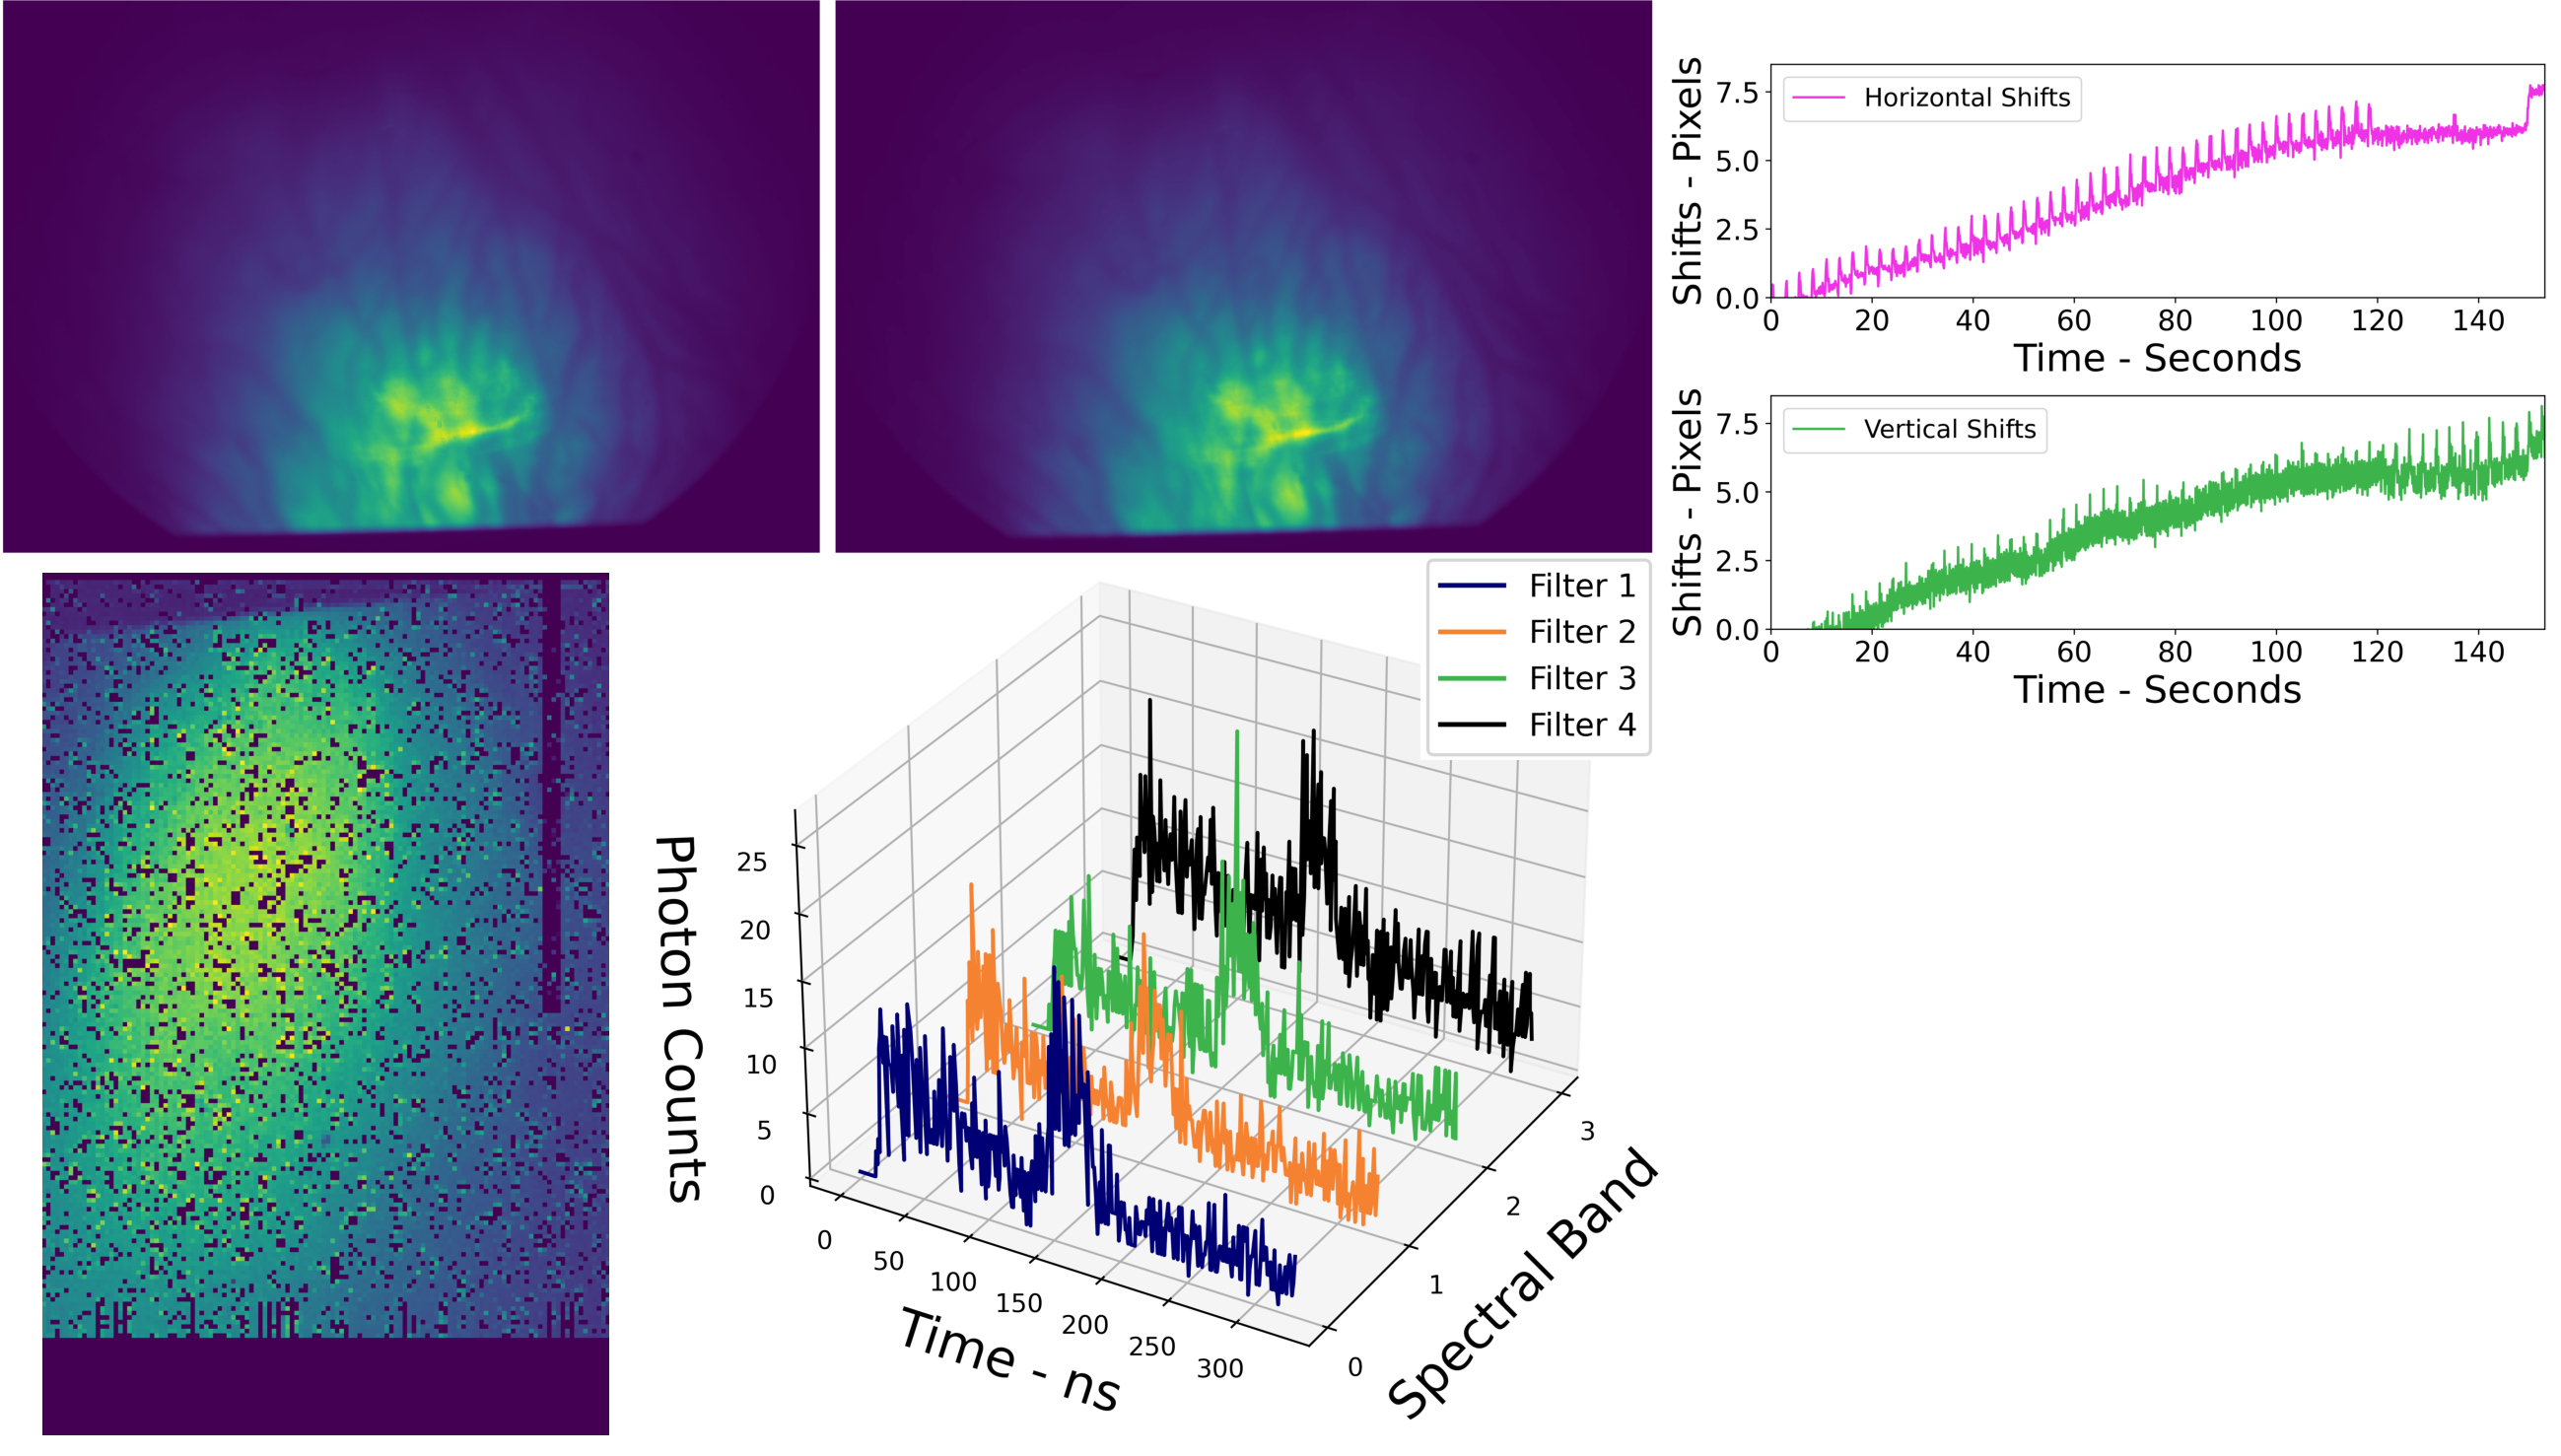
\includegraphics[width = \textwidth]{figures/ratUCL/ThesisFigure-Rat1RawData.pdf}}
%     \annotatedFigureText{0.01,0.945}{white}{0.3}{a)}
%     \annotatedFigureText{0.335,0.945}{white}{0.3}{b)}
%     \annotatedFigureText{0.665,0.945}{black}{0.3}{c)}
%     \annotatedFigureText{0.025,0.545}{white}{0.3}{d)}
%     \annotatedFigureText{0.3,0.55}{black}{0.3}{e)}
%     \end{annotatedFigure}
    
%     \caption{Caption}
%     \label{fig:rat1rawdata}
% \end{figure}

\subsection{Darkfield Correction}
In the histo

\section{Results For Rat 1, Day 2}\label{sec:rat1day2results}

\section{Results For Rat 2}\label{sec:rat2results}

\section{Summary Of Results}

textwidth in inches: \printinunitsof{in}\prntlen{\textwidth}